\scanpage{5}

\[\begin{array}{ccc}
p_0/p_1&\deleted{p_{12}\quad p_{23}\quad p_{31}}&\deleted{\delta_1\quad\delta_2\quad\delta_3}\\
\delta_0&\deleted{\deleted{\unsure{\sigma p_{12}\quad\sigma p}}}&\\
&\deleted{p_{21}\quad p_{32}\quad p_{13}}&
\end{array}\]
\mspage{\textcircled{2}}
\[\deleted{\delta_0p_0},\deleted{\delta_0p_1},\quad\mathrm{id},\sigma\]
\diagram{\begin{tikzpicture}[x=.009cm,y=-.009cm,line cap=round,line join=round]
\node at (113,251) {$E_0$};
\node at (326,240) {$E_1$};
\node at (527,221) {$\overset{\unsure{\prime|\cdot}}{E}_2$};
\node at (312,123) {\large$\mathcal G_2$};
\node at (526,105) {\large$\mathcal G_3$};
\draw[line width=.8pt] (283,233) -- (175,241);
\fill (175,241) -- (185,231) -- (183,240) -- (187,248) -- cycle;
\node at (215,196) {$p_0$};
\draw[line width=.8pt] (178,268) -- (284,263);
\fill (284,263) -- (274,254) -- (277,263) -- (273,273) -- cycle;
\node at (222,297) {$\delta_0$};
\draw[line width=.8pt] (491,209) -- (382,212);
\fill (382,212) -- (392,202) -- (389,212) -- (393,221) -- cycle;
\node at (444,166) {$p_{12}$};
\draw[line width=.8pt] (381,251) .. controls (420,267) and (455,267) .. (492,241);
\fill (492,241) -- (479,244) -- (486,246) -- (487,255) -- cycle;
\node at (440,296) {$\delta_1$};
\draw[line width=.65pt] (15,172) .. controls (1,172) and (9,158) .. (16,159)
 .. controls (65,155) and (137,153) .. (139,123)
 .. controls (137,97) and (131,70) .. (145,56)
 -- (655,15) -- (648,319) -- (634,325);
\draw[line width=.65pt] (20,191) -- (42,361)
 .. controls (260,350) and (470,344) .. (615,337);
\end{tikzpicture}}
\[\deleted{\delta_1p_{12}}\]
\diagram{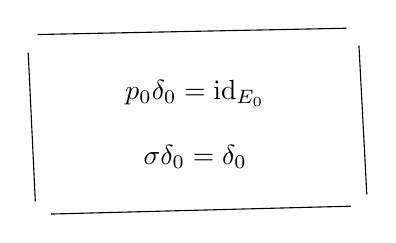
\begin{tikzpicture}[x=1cm,y=1cm]
\node at (0,.35) {$p_0\delta_0=\mathrm{id}_{E_0}$};
\node at (0,-.45) {$\sigma\delta_0=\delta_0$};
\draw (-2,1.1)--(1.92,1.18);
\draw (-2.12,.87)--(-2.03,-1.02);
\draw (2.08,.96)--(2.18,-.93);
\draw (-1.83,-1.18)--(1.98,-1.08);
\end{tikzpicture}}
\diagram{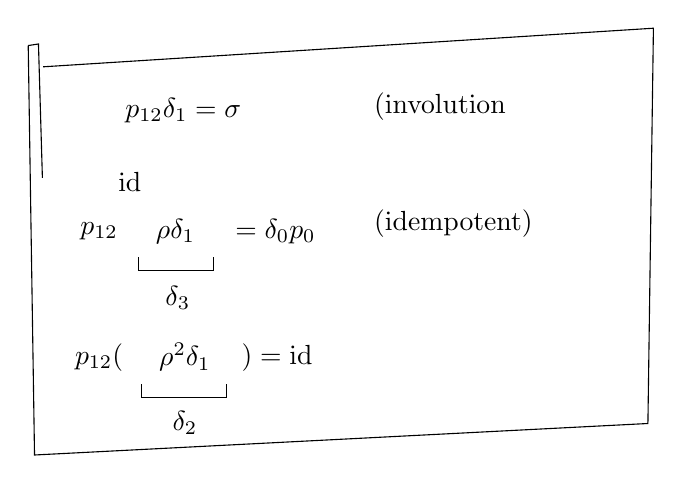
\begin{tikzpicture}[x=1cm,y=1cm]
\node at (-1.05,2.35) {$p_{12}\delta_1=\sigma$};
\node[anchor=west] at (1.25,2.4) {(involution};
\node at (-1.73,1.45) {$\deleted{\unsure{\mathrm{id}}}$};
\node at (-2.12,.82) {$p_{12}$};
\node at (-1.15,.82) {$\rho\delta_1$};
\node at (.12,.82) {$=\delta_0p_0$};
\node[anchor=west] at (1.25,.92) {(idempotent)};
\draw (-1.62,.49)--(-1.62,.32)--(-.67,.32)--(-.67,.49);
\node at (-1.12,-.02) {$\delta_3$};
\node at (-2.12,-.78) {$p_{12}($};
\node at (-1.03,-.78) {$\rho^2\delta_1$};
\node at (.14,-.78) {$)=\mathrm{id}$};
\draw (-1.58,-1.12)--(-1.58,-1.29)--(-.5,-1.29)--(-.5,-1.12);
\node at (-1.03,-1.61) {$\delta_2$};
\draw (-3.02,3.18)--(-2.94,-2.02)--(4.85,-1.62)--(4.92,3.4)--(-2.83,2.91);
\draw (-3.02,3.18)--(-2.89,3.2)--(-2.84,1.5);
\end{tikzpicture}}
\margin{\diagram{\deleted{\mbox{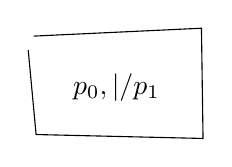
\begin{tikzpicture}[x=1cm,y=1cm]
\node at (0,0) {$p_0\unsure{,|/}p_1$};
\draw (-1.05,.65)--(1.08,.75)--(1.1,-.65)--(-1.02,-.6)--(-1.12,.47);
\end{tikzpicture}}}}
\diagram{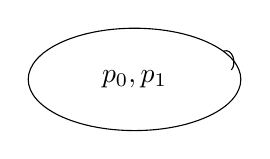
\begin{tikzpicture}[x=1cm,y=1cm]
\node at (0,0) {$p_0,p_1$};
\draw (0,0) ellipse[x radius=1.35,y radius=.65];
\draw (1.13,.36)..controls(1.25,.4)and(1.3,.2)..(1.23,.12);
\end{tikzpicture}}}
\diagram{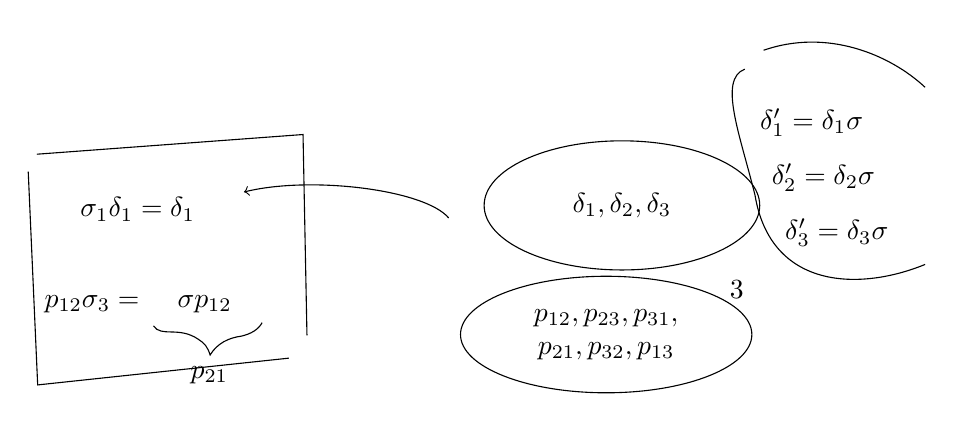
\begin{tikzpicture}[x=1cm,y=1cm]
\node at (-1.95,1.25) {$\sigma_1\delta_1=\delta_1$};
\node at (-2.53,.05) {$p_{12}\sigma_3=$};
\node at (-1.1,.05) {$\sigma p_{12}$};
\draw (-1.75,-.23)..controls(-1.65,-.38)and(-1.43,-.23)..(-1.18,-.4)
 ..controls(-1.1,-.45)and(-1.06,-.5)..(-1.03,-.6)
 ..controls(-.94,-.45)and(-.79,-.38)..(-.63,-.36)
 ..controls(-.51,-.33)and(-.42,-.28)..(-.37,-.19);
\node at (-1.04,-.86) {$p_{21}$};
\draw (-3.23,1.95)--(.15,2.2)--(.2,-.35);
\draw (-3.34,1.73)--(-3.22,-.98)--(-.03,-.64);
\draw[->] (2,1.14)..controls(1.7,1.5)and(.25,1.68)..(-.6,1.47);
\node at (4.2,1.3) {$\delta_1,\delta_2,\delta_3$};
\draw (4.2,1.3) ellipse[x radius=1.75,y radius=.82];
\node[align=center] at (4,-.34) {$p_{12},p_{23},p_{31},$\\$p_{21},p_{32},p_{13}$};
\draw (4,-.34) ellipse[x radius=1.85,y radius=.74];
\node at (5.66,.23) {$\unsure{3}$};
\node[anchor=west] at (5.83,2.35) {$\delta'_1=\delta_1\sigma$};
\node[anchor=west] at (5.98,1.65) {$\delta'_2=\delta_2\sigma$};
\node[anchor=west] at (6.15,.95) {$\delta'_3=\delta_3\sigma$};
\draw (6,3.27)..controls(6.8,3.55)and(7.6,3.22)..(8.05,2.8);
\draw (5.76,3.03)..controls(5.42,2.9)and(5.7,2.2)..(5.89,1.43)
 ..controls(6.09,.23)and(7.22,.21)..(8.05,.55);
\end{tikzpicture}}
\diagram{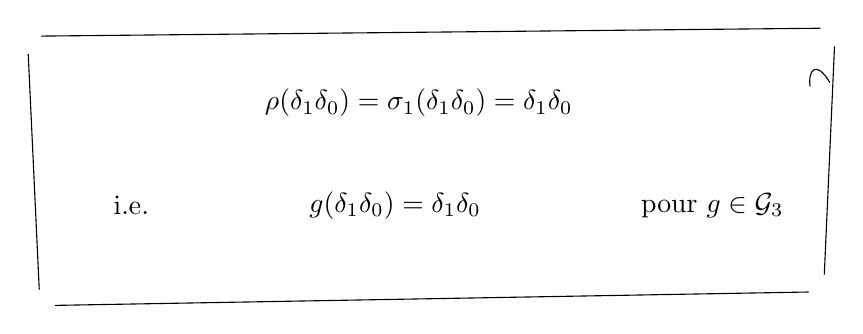
\begin{tikzpicture}[x=1cm,y=1cm]
\node at (0,1.1) {$\rho(\delta_1\delta_0)=\sigma_1(\delta_1\delta_0)=\delta_1\delta_0$};
\node[anchor=west] at (-4,-.2) {i.e.};
\node at (-.3,-.2) {$g(\delta_1\delta_0)=\delta_1\delta_0$};
\node[anchor=west] at (2.7,-.2) {pour $g\in\mathcal G_3$};
\draw (-4.8,1.95)--(5.1,2.05);
\draw (-4.96,1.72)--(-4.82,-1.27);
\draw (5.28,1.82)--(5.15,-1.08);
\draw (5.22,1.36)..controls(5.05,1.65)and(4.94,1.52)..(4.97,1.31);
\draw (-4.62,-1.47)--(4.95,-1.3);
\end{tikzpicture}}
\diagram{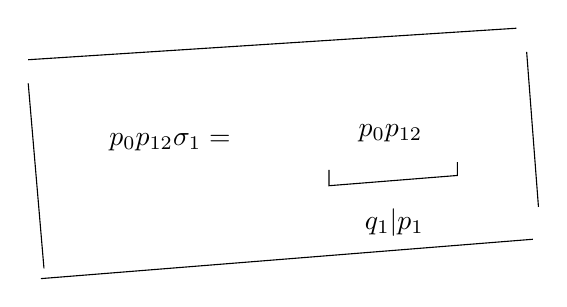
\begin{tikzpicture}[x=1cm,y=1cm]
\node at (-1.3,.45) {$p_0p_{12}\sigma_1=$};
\node at (1.5,.57) {$p_0p_{12}$};
\draw (.72,.1)--(.72,-.1)--(2.35,.03)--(2.35,.2);
\node at (1.55,-.57) {$\unsure{q_1|p_1}$};
\draw (-3.1,1.5)--(3.1,1.9);
\draw (-3.1,1.2)--(-2.9,-1.15);
\draw (3.23,1.6)--(3.38,-.37);
\draw (-2.94,-1.28)--(3.31,-.78);
\end{tikzpicture}}
\margin{\diagram{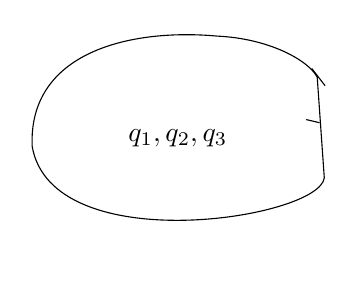
\begin{tikzpicture}[x=1cm,y=1cm]
\node at (0,0) {$q_1,q_2,q_3$};
\draw (-1.85,-.1)..controls(-1.9,1.1)and(-.6,1.4)..(.5,1.3)
 ..controls(1.15,1.27)and(1.65,1)..(1.77,.78)
 --(1.86,-.5)..controls(1.8,-1.02)and(-1.6,-1.55)..(-1.85,-.1);
\draw (1.7,.89)--(1.87,.67);
\draw (1.8,.2)--(1.63,.24);
\end{tikzpicture}}}
\margin{4}

